\documentclass[10pt,a4paper]{article}
\usepackage[utf8]{inputenc}
\usepackage{amsmath}
\usepackage{amsfonts}
\usepackage{amssymb}
\usepackage{graphicx}
\usepackage{bm}
\usepackage{wrapfig}
\usepackage{appendix}
\usepackage{subcaption}
\usepackage{framed}

% Sets small roman numerals as the symbols in enumerate environments
\usepackage{enumerate}
\usepackage{enumitem}
\setlist[enumerate,1]{label={\upshape(\roman*)}}

% Theorem environments
\usepackage[framed,standard]{ntheorem}
\theoremindent1cm
\newtheorem{assumption}{Assumption}
%\newtheorem{theorem}{Theorem}[section]
%\newtheorem{lemma}[theorem]{Lemma}
\newframedtheorem{algorithm}{Algorithm}

% Code formatting
\usepackage{listings}
\usepackage{color}
\lstdefinestyle{matlab_custom}{
	language = matlab,
	basicstyle=\scriptsize\fontfamily{cm}\sffamily,
	showstringspaces = false,
}

\usepackage[margin=2cm]{geometry} %Set margin size

\usepackage{fancyhdr}

\pagestyle{fancy}
\fancyhf{}
\rhead{Hanna Autio}
\lhead{\today}
\chead{Masters Thesis} %Course name

\cfoot{\thepage}

\usepackage{cleveref}
\crefname{assumption}{assumption}{assumptions}
\Crefname{assumption}{Assumption}{Assumptions}

\author{Hanna Autio}
\title{A stochastic model for Meningococcal Disease in the African Meningitis belt} %Title here
\date{\today}

\begin{document}
\maketitle
\thispagestyle{empty}
\cleardoublepage
\newpage
\setcounter{page}{1}

% On my indices:
% 	- Greek letters are constants
% 	- n \eta for populations
% 	- k \kappa for events


\section{Introduction}

The mathematical description of populations and disease dynamics is a field which can be extremely complex. It is a subject of much research, relevant to policy makers and medical researchers. An accurate model that can predict future dynamics can be of immense value, both to prepare for and deal with epidemics, and to evaluate different vaccination policies. However, accuracy in itself is not enough. The model must also be precise enough, as well as capable of evaluating several possible scenarios within a reasonable time frame. This leads to a need for a balance between accuracy, which means several different interactions must be considered, and swiftness, which calls for approximations and numerical efficiency.

A common practise for population dynamics is to approximate a discrete and random system, according to the central limit theorem and the law of large numbers, by a continuous and deterministic system. It is obvious that in a given population, the number of individuals is a discrete number. Furthermore, it is intuitively clear that events such as contagion and infection are fundamentally random. However, models that incorporate this randomness into their structure are in general significantly slower to use, as a single evaluation will take longer and more evaluations are needed to increase precision and accuracy (in correspondence to the Monte Carlo framework). Consequently, an approximation is made to a deterministic system governed by differential equations, and letting the populations vary continuously. By the law of large numbers and the central limit theorem, this is no issue if the population is large enough and a continuous population will, while not entirely accurate, be at least as specific as a realisation of a discrete random system. With this framework standard numerical procedures can be used, and as the model is deterministic only one evaluation is needed. However, the law of large numbers only holds as long as there is indeed a large number of individuals; whenever a population (or subpopulation) faces extinction the rule no longer holds. These and other factors must all be considered when determining what framework and what model is the most appropriate for the system at hand, with respect to accuracy, speed and likely system states.

Most classical approaches to population dynamics describes the system in terms of the relative number of individuals in a given sub-population, but there are some limitations to this method and alternatives should be considered. SIR-models and other compartmental models are examples of the aforementioned, where the system state is recorded based on how large the different population compartments are. However, in some cases this will not provide sufficient information. Consider for example the case where a model is used to estimate what capacity a maternity ward should have some years into the future. It is then not sufficient to consider only the population growth over time, but the raw number of births are the relevant factor. A compartmental model is not suited for this specific problem, and a model more focused on the specific dynamics should be developed.

The complexity in modelling population dynamics arises from several factors. Firstly, the modelling of a population in itself, disregarding external factors, can be made increasingly complex by considering each individual and the exact changes they are subject to. Secondly, external factors should be considered so as to make the modelling relevant for policy makers. What external factors to include and how precisely they should be modelled, as well as their precise effects on the population, introduces a whole new layer of complexity. For example, one external factor that may be interesting to consider is weather, and currently there is no reasonable way to reliably model the weather. It can even be argued that to accurately model a population, the whole system that is the earth itself must be considered. Consequently, some approximations and assumptions will be made, even when choosing the stochastic approach to modelling. As the stochastic approach is in general more complex, it can be argued that more of these assumptions and approximations will be made than in a corresponding deterministic model to compensate for the increased complexity otherwise. This should also be considered when evaluating different options for modelling.

The goals of modelling diseases can be many. There is obviously an interest in understanding and explaining the dynamics of the disease itself, to increase knowledge about the disease and potentially understanding the underlying biological mechanisms. It can also be used as a validation tool to confirm or dismiss theories about a disease, if the model and simulation method is proven sound beforehand. One of the more relevant and obvious goals of these models is to help policy makers determine what the consequences of different actions can be in different circumstances. This will help showing whether a vaccination policy is efficient, or what the best cause of action during an epidemic may be. Furthermore, as there are frequently issues in gathering real-world data, a reliable model can provide more and higher-quality data that can later be used to identify dynamics that could, for example, be used as a predictor for future epidemics.

For the reasons mentioned above, it is important that a given model is flexible. The framework must not only support different scenarios in the disease dynamics itself, but it should also support variations in external policies, corresponding to several different policies but also to variations in the resources controlled by the policy makers. This is especially important when modelling populations in areas of the world with poor infrastructure, as this can affect the data available as well as the possible responses from medical personnel and governments.

A flexible and reliable model should also be able to adapt to changes within the community themselves. For many diseases, including for example measles, there is a clear pattern of disease corresponding to population movements and population mixing[Spatial patterns of...]. These mechanisms can lead to an increased rate of transmission, as populations grow, or the introduction of new disease variations to groups with lacking immunity or poor preparations in other ways.

Where the infrastructure is poor, a plethora of new issues arise. There are often issues with distributing drugs and vaccines, meaning that any policy will be less efficient. This also increases the need for an early warning, as the time it takes to react to a given scenario increases. Furthermore, there can be issues considering the gathering of information itself. If sick individuals can not reach a medical institution in time, or if the information from the medical institutions take too long to spread, the true situation will be unknown. These are factors that should be considered when using models as an aid for political decisions, but it should also be considered when constructing the model itself.

In this project, a stochastic and discrete model for the dynamics of Meningococcal disease in the African Meningitis belt is constructed and evaluated. The model is then used to examine dynamics of the disease, as well as to examine some possible explanations for the dynamics in question.

Meningococcal disease are any diseases caused by \emph{Neisseria Meningitidis}. The infection of N. Meningitidis can take many forms, of which two common (and severe) are meningococcal septicaemia and meningitis [source]. Meningitis is an infection of the thin lining surrounding the brain and the spinal cord, and is a serious condition that untreated leads to death in about 50\% of cases. Early diagnosis and adequate treatment reduces the fatality rate to about 5-10\%, with permanent disabilities in about 10-20\% of cases. The incubation time varies from 2-10 days, but is on average 4 days [source: WHO]. Meningococcal septicaemia is the infection of the bloodstream, and is often even more severe than meningitis. The infection damages the walls of blood vessels and leads to bleeding into the skin and other organs. The treatment is similar, but possible consequences include amputation[source]. In rare cases, N. Meningitidis can cause arthritis and similar diseases[source].

Humans are the only known reservoir for N. Meningitidis. At a given time, about 2-50\% of the population are likely to be carriers of the bacterium, and it is spread by salivary droplets. Carriage can last both for a very short period of time as well as for several months, during which the bacterium is present in the nasopharynx of the carrier \cite{taha2002duality}. In general, carriage does not lead to invasive disease, but it has been linked to a subsequent immune response to the bacterium. There are several mechanisms that can participate in the immune response, and research has shown that a significant part of the adult population have an immune response that is putatively protective towards the disease [source: human immunity to the meningococcus]. Another bacterium frequently theorized as potentially leading to immunity to the disease is \emph{Neisseria Lactamica}, often present in the nasopharynx of young children [source]. While immunity protects towards invasive disease, it has not been shown that there is any reduction of carriage caused by the immune response. [sources]

\emph{N. Meningitidis} is genetically variable. It is most commonly classified based on the composition of its polysaccharide capsule into 13 different serogroups. While it is rather common, world-wide, for carriage strains to not have a capsule (around 50\% of carriage cases), and thus be non-serogroupable, disease is primarily caused by encapsulated strains. Serogroups A, B, C, W135 and X account for more than 90\% of cases of invasive disease world wide. The production of a capsule can be switched on and off with high frequency, and also non-serogroupable carriage strains can be pathogenic. [NM an overview..].

The African meningitis belt is a region in Sub-Saharan Africa with an increased rate of meningococcal disease as well as recurring epidemics. The belt was first described by Lapeyssonnie in 1968 \cite{lapeyssonnie}. This region is shown in \cref{[FIGURE:MENINGITIS BELT]} and has been characterized by semi-regular epidemics documented since the early 20th century. Its specific geographical area is defined be the WHO as the region in Africa between Senegal in the west and Ethiopia in the east [source], which coincides fairly well with the area described by Lapeyssonnie.

Meningitis dynamics in the region have, among others, these characteristics. Firstly, there are recurring epidemics with intervals of about 5-15 years. Secondly, the incidence rates of disease is higher than in other regions of the world. Thirdly, the disease is most commonly caused by a serogroup which does not usually cause epidemics in the rest of the world. All of these properties are also affected by a strong seasonality, so that there are three distinguishable states for the disease in a population. There is the hypoendemic state, with a low incidence rate of about [] which occurs during the wet season. During the dry season, the system falls into a hyperendemic state with increased incidence rate, or occasionally an epidemic state. An epidemic state is defined as a rate of disease above []. \cite{mueller2010hypothetical}

The reason for the specific dynamics in this region is often considered to be related to climatic factors. One such factor frequently considered is the total precipitation. The region coincides fairly well with the area between the 300mm and 1100mm isohyets \cite{molesworth2002meningitis}. Another common climate factor for the area, is that it is affected by the Harmattan, a dry wind from the Sahara desert. As there are links between factors that irritate the airways and subsequent infection by \emph{N. Meningitidis} [sources on smoking, colds], a link between the Harmattan and the hyperendemic meningitis season would seem plausible. Is is an area of active research [?], and finding any climactic factors that could be driving the epidemics is outlined as an area of priority by the WHO [source: research priorities].

The distribution of genetic variations of \emph{N. Meninigitidis} is different in the meningitis belt compared to the rest of the world. There is a higher ratio of encapsulated virulent strains carried in the population, most notably of serogroup A. This serogroup has also been the cause of most epidemics in the region. Furthermore, there is significantly less genetic variation in the population that in other regions. The temporal distribution of the bacterium is also unstable, leading to a clonal wave pattern, where one strain is dominant at a given time. [clonal waves]. It has been theorized that this lack of genetic variation can contribute to the epidemic patterns, as an epidemic strain can quickly become dominant and out-compete less virulent strains. The reasons for the lack of stability and lack of variation is unclear.

There is a clear relationship between age and the distribution of carriage and disease caused by \emph{N. Meningitidis}. Globally, the carriage rates are around 10\% in an endemic state, but the rate is significantly lower ($<3\%$) for young children, and significantly higher for teenagers and young adults, especially for military recruits and university students ($>24\%$). Other factors that correlate with increased carriage are smoking and crowding, for example at bars or during the Hajj [Epidemic meningitis...]. The significant increase in carriage in closed communities such as the military, the Hajj or to some extent new university students suggest that population mixing may be related to the transmission of disease.

The group at most risk for disease are young children, in connection with waning maternal immunity. There is also an increased risk in teenagers and young adults, similar to the increase in carriage rates for these groups.

Vaccines against the bacterium have historically been focused primarily on antigens found in the capsule, called polysaccharide vaccines. These vaccines have been used to prevent invasive disease in individuals older than infants, but does not induce an immunological memory. As such, preventative vaccine policies can not efficiently be carried out using these types of vaccines. Recently, polysaccharide conjugate vaccines have been introduced, which are capable of inducing immunological memory as well as immunizing infants. These conjugate vaccines currently exist for serogroups A and C. There have been indications that carriage of the targeted strain decreases following a conjugate vaccine intervention. However, it is unclear whether this is caused by a decrease in carriage of the strain itself or only prevents the production of the capsule. [NM an overview]

Since 2010, a WHO project has been undertaken to combat epidemic meningitis in the region. A polysaccharide-conjugate vaccine effective against serogroup A has been introduced, and since its introduction, no new epidemics has been recorded from that specific strain. There are also indications that the vaccine affects carriage rates of the specific strain, which could lead to herd immunity. These types of effects has been seen in other vaccination projects against N. Meningitidis [sources], but the effects on the specific dynamics in the Meningitis belt is yet unclear. One concern is whether the eradication of serogroup A could lead to an increase in other serogroups, specifically those with a higher virality.

A [recent] conference on the Meningitis belt outlined a few priorities for future research, where it was determined that attempts to construct mathematical models should include factors that may affect the spatial, seasonal and year-to-year variability in risk for meningococcal disease. The model constructed in this project focuses on the seasonal variability, and examines two different explanatory models for the variations. The year-to-year variability will also be examined to a certain extent, as variations in the population distribution over time could lead to long-term variability in risks for disease and epidemics.

This model is also the first, to my knowledge, stochastic model for Meningococcal meningitis in the African Meningitis belt. As much of the region has a low urbanization rate, a model suitable for smaller populations is appropriate. Furthermore, as the incidence rates during the endemic season can be very low there are clearly situations where the law of large numbers may not hold. This model could be used to verify previous modelling attempts, as well as evaluate current theories on the underlying causes of epidemiological dynamics.

\subsection{Main goals of this project}

The primary goal of this project has been to create and implement stochastic model for the population and disease dynamics in the African Meningitis belt. The model should be evaluated, and its calculations should be compared to real-world data and other models, to determine whether there is an improvement in the accuracy and specificity of the model.

If the model and its implementation seems sound, some further questions are to be considered. The primary consideration of this thesis is to attempt to determine whether the difference between the endemic and the hyperendemic states of the disease can be explained by behavioural changes or whether the explanation must be found somewhere else, for example in biochemical factors of the bacterium itself.

To further determine the seasonality of the disease, also the epidemic state should be considered. While epidemic outbreaks are connected to the introduction of a more invasive strain, the epidemics themselves also display a certain seasonality. Using the seasonal variations found to produce the most accurate results in the previous section, the results of introducing a more invasive strain during different seasons will be examined. If the introduction leads to an epidemic also during the wet season, or fails to lead to an epidemic in the dry season, the suggested explanation does not hold.

% What are the goals of this thesis and why have I chosen to focus on those aspects?

%\subsection{Terminology}
% Event
% System
% probability rate
% population/subpopulation

\section{Methods}

The development of a stochastic model for population dynamics aims at determining the probability for the system to be in a given state at a given time. Typically, there will not be a closed-form analytical solution for this problem, and the Monte Carlo framework is employed to produce estimates. This is also the basic method used in this project. This means that a model is developed for the general, stochastic behaviour of the system, and a multitude of realisations are simulated. The aggregate of these realisations should then be a viable approximation of the probabilistic behaviour of the system.

For this problem, it was determined that a model should not focus only on the population distribution over time but also the number of times any individual was infected. There are several reasons for this; One is that the rate of permanent sequelae is significant, meaning that while an individual may recover from the disease itself the history of their disease is still relevant. Another reason is that the information used to determine when an epidemic is, is the number of cases that has occurred and not the specific number of sick individuals at a given time. These factors leads us to construct a model that focuses on the dynamics of the system.

In this section, we first explain the model constructed for this problem and the theory behind the algorithm used to construct realisations. Then follows a section on the implementation, both from a mathematical standpoint and a computational, and finally a section discussing the real-world data and parameters used in the project.

%
%
%The goal of this project is to develop methods to understand the dynamics characterizing meningococcal disease in the meningitis belt. The degree of urbanization is comparatively low in this region [source] and so any applicable method must be accurate also for smaller communities. As discussed in the introduction, traditional methods using deterministic dynamics and non-discrete populations become gradually more imprecise when dealing with decreasing population sizes [source], and so a different approach is used. We develop a dynamical model for integer-valued populations following a Markov-Jump process. The model is subsequently simulated using the Feller-Kendall algorithm, and its behaviour is validated by comparing to real-world data as well as to previous models (on an appropriate scale).

% Make a comparison to earlier modelling examples and comment on why they may be less accurate

\subsection{Model} \label{section:model}

According to the comments made above, a stochastic model focusing on the relevant dynamics was created. We begin by defining what dynamics should be considered, and constructing classes of events corresponding to each type of dynamic. For example, we will consider dynamics such as transmission and recovery and define one event class for each of these. Using this framework, we can record the number of times an event of each class occurs and take it as the system state variable. Given $m$ event classes, the system state variable at time $t$ is the vector $\bm{N}\left( t \right) = \left[ N_1 \left( t \right), \ldots, N_m \left( t \right) \right], \textrm{ each }N_\mu \in \mathbb{N}$. The ultimate goal is to determine the probability $P \left( \bm{N}\left( t \right)  = \bm{n} | X\left( \bm{0} \right) \right)$ or: The probability that precisely $\bm{n} = \left[ n_1, \ldots, n_m \right]$ events of each class has occurred at time $t$, given an initial population space $X_0$.

The population space is constructed by choosing a particular population and compartmentalising it into $k$ sub-populations, similarly to the methodology of classical SIR-models. The compartmentalisation should be such that no individual can be included in more than one sub-population at a time, and no event should increase or decrease a given sub-population by more than one. The compartmentalisation used in this project is shown in \cref{fig:population_flow} and further discussed in \cref{section:populations}. The population space at time $t$, $X_t$ is a k-dimensional stochastic variable. Later we will discuss its dependence on the event counts $N \left( t \right)$.

The event $N\left( t \right)$ counts form an m-dimensional stochastic process, which under the following assumptions is a density dependent Markov Jump process.

\begin{assumption} For a sufficiently small time interval $h$, the following assumptions hold:
	\begin{enumerate}
		\item Event occurrences in disjoint time-intervals are independent \label{assumption_1a}

		\item The Chapman-Kolmogorov equation \cite{Kolmogoroff1931,Feller1940} holds.  \label{assumption_1b}

		\item $P\left( N_{\mu} \left( t  + h \right)  - N_{\mu} \left( t \right) = 1 | X_t \right) = W_{\mu} \left( X_t \right) h + \mathcal{O} \left( h \right)$. \label{assumption_1c}
	
		\item $P\left( N_{\mu}\left( t+h\right) = N_{\mu} \left( t \right) | X_t \right) = 1-W_{\mu}\left( X_t \right) h + \mathcal{O}\left( h \right)$. \label{assumption_1d}

		\item $P\left( N_{\mu}\left( t + h \right ) - N_{\mu} \left( t \right) = k | X_t \right)= \mathcal{O}\left( h \right) , \, \textrm{ for all } k \geq 2$. \label{assumption_1e}
	\end{enumerate} \label{assumption_1}
\end{assumption}

\Crefrange{assumption_1c}{assumption_1d} in \cref{assumption_1} implies that the process formed by the event counts for a single class is a Poisson process with rate $W_{\mu}$. We assume each $W_{\mu}$ is a smooth function of the population. Assumption \ref{assumption_1e} ensures that no more than one event can occur simultaneously. Note also that conditioning the probabilities on the population $X_t$ at $t$ is sufficient, although conditioning based on the event counts $N\left( t \right)$ and the initial population state would also hold in this context.

% Discuss some properties of a Poisson process

The Chapman-Kolmogorov equation is as follows: Consider a stochastic process $\xi_1, \ldots, \xi_k$, with a joint probability density function $p_{\xi_1 \ldots \xi_k} \left( x_1, \ldots, x_k \right)$. Then the probability density
\begin{align*}
p_{\xi_1, \ldots, \xi_ {k-1}} \left( x_1, \ldots x_{k-1} \right) = \int_{-\infty}^\infty p_{\xi_1, \ldots, \xi_k}\left( x_1, \ldots, x_k \right) \mathrm{d} x_k,
\end{align*}

corresponding to a straight-forward marginalisation of the joint probability density function.

Now, we consider the dependence of the population space on the event space. For each event class $\mu$ we define a vector $\delta^\mu$, where $\delta^\mu_\kappa$ describes the effects of event $\mu$ on population $\kappa$. The eventcounts can then easily be mapped to the population space by constructing a matrix $\bm{\delta} = \left[ \delta^1 \ldots \delta^m \right]^{T}$ as $X_t = X_0 + \bm{\delta} \bm{N} \left( t \right)$, but note that some information is lost in this projection. Using this description, there are no changes in the population outside of the events, which should match the initial idea that all relevant dynamics should be modelled using the event framework.

% Maybe add some comments discussing how the population at time t and t+h are dependent, while the same does not hold for the events occurring in the different segments.

Earlier we mentioned that the process constructed is a density dependent Markov jump process. The jump aspect of the process is in the discrete nature of the event counts, meaning that the system state jumps from one state to another with the instantaneous occurrence of an event. The density dependence is introduced via the probability rates $W_\mu \left( X_t\right)$, as they describe the future evolution of the process based on the current population and the current system state. Then only the Markov property should receive some further consideration. Again, we look to the $W_\mu$. They depend on the population state (and consequently the system state) $X$ at time $t$, but not on any earlier state. This is precisely the Markov property.

In the comments on \cref{assumption_1}, we mentioned that each event count formed a Poisson process, so that the aggregate event counts forms a multivariate Poisson process. A well-known result for these is the following:

\begin{lemma} \label{lemma:exponential}
	The waiting time $H$ to the next event is exponentially distributed with a rate $W = \sum_{\mu=1}^m W_\mu$
\end{lemma}

This result will be used later, and so we will prove it here:

\begin{proof}
	The waiting time to the next event is given by the time until the very next event occurs. Let $H_\mu$ be the waiting time until event $\mu$. Then	$H = \min \{ H_1, \ldots, H_m \}$ or equivalently $H_\mu \geq H \textrm{ for all } \mu$. Given the system state at time $t$, the events can be regarded as independent. This gives us the following probability density function for $H$, where we use that $H_\mu \sim \exp \left( W_\mu \right)$:
	\begin{align*}
		f_{H} \left( h \right) = \prod_{\mu = 1}^m P \left( H_\mu \geq h \right) = \prod_{\mu =1}^m 1 - F_{H_\mu}\left( h \right) \underset{h\geq 0}{=\joinrel=} \prod_{\mu = 1}^m \mathrm{e}^{-W_{\mu} h} = \mathrm{e}^{- h \sum_{\mu = 1}^m W_\mu}
	\end{align*}
	This is precisely the exponential probability density function, with parameter $\sum_{\mu = 1}^m W_\mu$.
\end{proof}

Another result concerns the time-evolution of the probabilities governing the system state:

\begin{theorem}
	Under the previous assumptions, the dynamics in the event space obeys the Kolmogorov Forward equation.
	
	\begin{align}
		\frac{\textrm{d}}{\textrm{d}t} P \left( N \left( t + s \right) = \bm{n} | X_t \right) =
		&  \sum_{\mu = 1}^m P \left( N \left( t + s \right) = \left[ n_1 \ldots n_\mu - 1 \ldots n_m \right] \right) W_{\mu} \left( X_ {t+s} - \delta^{\mu} \right) - \\
		- & \sum_{\mu = 1}^m P \left( N \left( t + s \right) = \bm{n} \right) W_{\mu} \left( X_{t+s} \right) \label{eq:kolmogorov_forward}
	\end{align} \label{th:kolmogorov_forward}
\end{theorem}

where we have used $X_{t+s}$ to mean $X_0 + \bm{\delta}\bm{n}$, or the population state given the event counts $\bm{n}$. The interpretation of the equation is as follows: The probability that a function should be in a given state at a given time increases as the probability that it should enter the state increases, and decreases as the probability that it should leave that state increases. The first term corresponds to the probability that it should enter the given state, as it is the probability that it should be in an immediately preceding state and enter the given state. The second term is interpreted similarly.

\Cref{th:kolmogorov_forward} provides us with a differential equation describing the probability distribution evolution for the event counts, but in general there are no simple solutions to it. Instead we look to an approximate solution using the Monte Carlo-framework, meaning we construct many artificial "samples" of the stochastic variable $N \left( t \right)$, and assume that the distribution of the samples can be used as an approximation for the distribution itself. This requires us to find an effective method of simulating a system as the one we have described, and one such method is the Feller-Kendall algorithm, also known as the Gillespie algorithm [citations].

To construct a realisation of the system, we will work iteratively and use the fact that the system state is constant between events. This means that the only times we are interested in are the times where an event occurs. Furthermore, we are only interested in the very next event, as that event may change the probability distributions for future events. Consequently, in order to move the realisation forward in time, the stochastic variables we would like to sample from are the time of the next event, $H$ and what event it is that occurs, $M$. An initial idea for sampling these variables together is the following:

\begin{algorithm} Let the system be in state $N$ at time $t$, with populations $X$. \label{algorithm:bad}
	\begin{enumerate}
		\item Calculate the probability rates $W_\mu \left( X \right)$
		\item Sample times $H_\mu$ for the time of the next event of each event class
		\item Choose the event class $M$ so that $H_M = \min \{ H_1, \ldots, H_m \}$
		\item Increase the event count of $M$ by one:
			\begin{align*}
				N := \left[ N_1\left(t \right) \ldots N_M \left( t \right) + 1 \ldots N_m \right]
			\end{align*}
		\item Update the time and the population:
			\begin{align*}
				X := X + \bm{\delta}^{M} \\
				t := t + H_M
			\end{align*}
		\item Repeat
	\end{enumerate}
\end{algorithm}

This algorithm will work, but is not very efficient. In each step, $m$ random numbers are generated, of which $m-1$ are discarded. If the event count is high, this can lead to a significant increase in simulation time on each step. Instead, we will use the following result:

\begin{lemma} \label{lemma:independence} % Source: p129 in Durretts "Essentials of stochastic processes", 2010
	$M$ and $H$ are independent.
\end{lemma}

In order to prove this, we will use the definition of independence: $P \left( A \cap B \right) = P \left( A \right) \cdot P \left( B \right)$. We will determine the joint probability density function of $(H, M)$ and show that this is the product of the marginal distributions.

\begin{proof}
	First, we consider the marginal distributions. In \cref{lemma:exponential}, we showed that $H \sim \exp \left( \sum_{\mu = 1}^m W_\mu \right)$. We now consider the distribution of $M$, by first studying the case where there are two exponentially distributed independent variables and generalising. Let $S \sim \exp \left( \lambda_S \right), T \sim \exp \left( \lambda_T \right)$ be independent. We will determine the probability that $S$ occurs before $T$, or $P ( S < T )$. Using independence and the exponential distribution, we get:
	
	\begin{align}
		P \left( S < T \right) = \int_0^\infty P ( S = s) P (T > s) \mathrm{d}s = \int_0^\infty \lambda_S \mathrm{e}^{- \lambda_S s} \mathrm{e}^{-\lambda_T s} \mathrm{d}s = \\
		= \frac{\lambda_S}{\lambda_S + \lambda_T} \int_0^\infty (\lambda_S + \lambda_T ) \mathrm{e}^{-(\lambda_S + \lambda_T)s} \mathrm{d}s = \frac{\lambda_S}{\lambda_S + \lambda_T}, \label{proof:independence_eq1}
	\end{align}
	showing that the probability that it should be a particular event is proportional to its rate. Now for the generalization: Consider a set of variables $T_j \sim \exp \left( \lambda_j \right), j = 1, \ldots, I$. Let $S = T_i$ and $U$ the minimum of the remaining variables. By the result from \cref{lemma:exponential}, $U \sim \exp ( \sum_{j \neq i} \lambda_j)$. Combining this with \cref{proof:independence_eq1}, we have
	\begin{align}
		P \left( T_i = \min \{ T_1, \ldots, T_I \} \right) = P \left( S < U \right) = \frac{\lambda_i}{\sum_{j = 1}^{I} \lambda_j},
	\end{align}
	implying that the marginal distribution for $M$ is proportional to the individual rates $W_\mu$.
	
	Now to compute the joint probability distribution for $(H, M)$.
	\begin{align*}
		P \left( H = h \cap M = \mu \right) = P \left( H_\mu = h, H_n > h \textrm{ for } n \neq \mu \right) = W_\mu \textrm{e}^{- W_\mu h} \prod_{n \neq \mu} \textrm{e}^{-W_\mu } = \\
		= W_\mu \textrm{e}^{- h \sum_{n=1}^m W_n} = \frac{W_\mu}{\sum_{n = 1}^m W_n} \left( \sum_{n=1}^m W_n \right) \textrm{e}^{-h\sum W_n},
	\end{align*}
	which is precisely the product of the probability density and distribution of $H, M$.  Hence they are independent.
\end{proof}

This result allows us to sample $H$ and $M$ separately from the marginal distributions defined above. The new algorithm is:

\begin{algorithm} Let the system be in state $N$ at time $t$, with populations $X$:
	\begin{enumerate}
		\item Calculate the probability rates $W_\mu \left( X \right)$ and use this to determine the distributions of $H$ and $M$
		\item Sample $H$ and $M$
		\item Increase the event count for class $M$ by one,
			\begin{align*}
				N := \left[ N_1 \left( t \right) \ldots N_{M} \left( t \right) + 1 \ldots N_m \left( t \right) \right]
			\end{align*}
		\item Update the time and the population:
			\begin{align*}
				t := t + H\\
				X := X + \bm{\delta}_M
			\end{align*}
		\item Repeat
	\end{enumerate} \label{algorithm:good}
\end{algorithm}

This method only requires two random variables to be sampled in each iteration, and is therefore significantly faster than the option presented in \cref{algorithm:bad}. This is the basic Feller-Kendall algorithm, and also the one used in this project.

% Introduce an example of one of the equations governing the rates. Probably one of the semi-complex.

\subsection{Implementation}

The first part of this section focused on how the model described above was applied to the specific problem discussed in this paper. The population compartmentalisation is explained, and an example of an equation for calculating the rates is given. Furthermore, the introduction of a time dependency is discussed. The second part focuses on the work to implement a computer program suitable for generating realisations of the system.


\subsubsection{Events and populations} \label{section:populations}

When constructing a compartmentalisation suitable for this problem, we start by considering what dynamics we want to model as events. We then construct the sub-populations in such a way that each event will increase one sub-population by one, decrease a sub-population by one, or both (moving a single individual from one population to another).

The types of dynamics that we want to model in this project can roughly be divided into two categories, dynamics relating to meningococcal disease and dynamics present in the healthy population. Due to the rather long intervals between the large-scale epidemics, it was determined that changes in the population distribution, as well as ageing individuals, could affect the model. This is the reason for including some dynamics of a healthy population, and finding a suitable approximation for the large-scale population variation over time was the first step.

The dynamics concerning a healthy population includes death by causes other than meningococcal disease, ageing and birth. The compartmentalisation and the events for a healthy population is shown in \cref{fig:healthy_pop}. The population is divided into three age groups, infants (0-4 years), young (5-14 years) and adult ($\geq15$ years), based on available data for the population and the disease. Death and birth was included in a slightly simplified manner. It was assumed that death only occurs in the oldest age group, and that only the oldest age group bear children. In order to compensate for the lack of infant mortality, the birth rate was based on the number of children that survive the first year.

Modelling meningococcal disease is the primary goal of this project, and as such much care must be put in determining what events and populations to include. The compartmentalisation and events relating to disease (for a single age group) are shown in \cref{fig:sick_pop}. A central part of the disease dynamics in this case is the presence of non-symptomatic carriers, and how this relates to transmission and immunity. Here, we choose to model the acquisition of carriage (on a susceptible individual) as a two-step process. We consider the event of transmission to a susceptible individual. This moves one individual from the sub-population "Susceptible" into a sub-population we call "Infected". Subsequently there is a second event, either one where the individual  becomes sick or one where they become a carrier. This event occurs on average 10 days after the transmission, corresponding to the incubation time for meningococcal disease. Carriers can then recover in one of two ways, either becoming immune to invasive disease or becoming susceptible. When it comes to transmission, we assume that carriers can transmit the bacterium to other individuals. We consider immunity to be protective against invasive disease, but not against carriage, so immune individuals can become carriers. In this case they never pass through the infected sub-population but are instead moved to the carrier population. This type of immune individuals can also lose immunity. However, when we consider individuals that recover from invasive disease they are always immune for the rest of their lives.

When we construct the events and the populations, the equations governing the events is also created. We assume that the rates follows the law of mass-action, so that the rate is proportional to the concentration of the relevant population. This also means we assume the population is perfectly mixed at all times, or (equivalently) that the population is evenly and randomly distributed in space. The equations for each event rate can be found in \cref{appendix:event_eqs}, but we will explain the basic idea behind them here using a (simplified) example. We will consider the transmission event to a susceptible individual, but for now we will not care about the different age groups. The generalisation is however straight-forward.

Consider an infective individual. In order for this individual to transmit disease, they must encounter a susceptible individual, and this encounter must also be sufficient to transmit bacteria. We call the expected number of contacts that lead to transmission per time unit and infective individual $\beta$. However, some of these contacts will be with non-susceptible individuals. As we expect the population to be evenly distributed, we can assume that the chance that a given individual is susceptible is equal to the relative number of susceptible individuals in the population, $\frac{S}{N}$ where $S$ is the number of susceptible individuals and $N$ the full population. This holds for each infective individual, which gives us the rate

\begin{align}
	W = I \beta \frac{S}{N} \label{eq:rate}
\end{align}

\subsubsection{Time dependency}

One of the main goals of this thesis is to examine possible explanations for the seasonal difference between the endemic and the hyperendemic state. In order to evaluate the effects of different mechanics, we introduce events with a time dependency, that intend to model different mechanics for different time periods. We let the probability rate for these events be zero during the season where they are not active. For this project, the activation and de-activation of these events are deterministic. The combination of these methods lead to discrete and deterministic seasonal shifts. The reason behind this choice is predominantly simplicity, but it also results in a system where the changes introduced by the shift in mechanics will be very clear and easy to compare.

Due to the nature of the algorithm we use (\cref{algorithm:good}), deterministic changes can be slightly complex to introduce. Time moves forward in discrete and random steps, meaning that the time introduction of the new event will never explicitly occur. We solve this by introducing the new events immediately following the first event after the pre-determined time. Provided events are frequent enough, this should not introduce any errors of more significance than the ones introduced by approximating the seasonality as an entirely deterministic process.

Two types of seasonal events were introduced, one intended to model a behavioural change in the population and one intended to model an external change in the disease itself. For the event concerning behavioural change, we will consider the specific dynamic where several, typically separate populations, are mixed due to migration or lack of resources. This is modelled by constructing a realisation of two separate populations in parallel and having a seasonal event corresponding to cross-transmission, where infective individuals in one population can transmit bacteria to individuals in the other population. When we consider a change in the disease itself, instead of introducing more events during the dry season, we will have one set of events during the dry season and another during the wet season. In general, the only reason between these sets will be in (some) of the parameters used in the equations governing the probability rates (see $\beta$ in \cref{eq:rate}). Predominantly we will consider a seasonal variation in the invasiveness parameter, that affects the probability that a susceptible individual that is infected by the bacterium becomes sick rather than becoming a carrier.

\subsubsection{Computer implementation}

The model was implemented in \verb0C++0, and the program could easily be adapted to a different problem. All analysis was performed in \verb0python0, using the \verb0numPy0 library.

Each model configuration was run 100 times. This was estimated to be enough to examine the general behaviour of the system, and to give an estimate of the expected behaviour. Furthermore, in cases where there are no notable deviations between realisations, we also assume the variations from realisation to realisation to be Gaussian distributed. This allows us to use standard methods for calculating confidence intervals.

\subsubsection{Data processing and analysis}
Scripts for analysing the data was written in \verb0Python0, using libraries \verb0NumPy0 and \verb0StatsModels0.

Most calculations are straight-forward estimates, using the arithmetic mean as an estimate of the expected value and the measurement variance as an estimate of the variance. Mean values was calculated using the \verb0NumPy0 mean function. 

When calculating incidence rates, data on the events was used. Initially it was differentiated to find the daily events data. In order to account for transient behaviours and only consider a steady state solution, the data from the first 2000 days of each realisation was discarded. Again, the arithmetic mean for all realisations was considered. The weekly incidence rates was calculated for each day (except the first six) as the sum of the average events the last seven days, including the current. Using this method, rather than dividing the sequence into weekly segments and summing over these, leads to more data points, but also means that the data points are not independent. This must be considered when estimating the statistical properties of the resulting values. In this report it is primarily relevant when calculating the variance of the mean estimate. We also note that enough data points are produced that the aggregate will be approximately Gaussian distributed. Using tools from time series statistics [source: an introduction...], the variance of the mean as an estimate of the expected value, for large enough data sets, is:

\begin{align*}
	\textrm{V} \left( \hat{m} \right) \approx \frac{1}{N} \sum_{k=-\infty}^{\infty} r_x \left( k \right)
\end{align*}

where $k$ are the lags, $r_x$ is the autocovariance function and $N$ is the number of available data points. The standard biased estimator for the autocovariance function supplied by \verb0StatsModels0 was used to find an estimate of $r_x$:

\begin{align*}
	\hat{r}_x \left( k \right) = \frac{1}{N} \sum_{t=k+1}^N \left( x_t - m \right) \left( x_{t-k} - m \right)
\end{align*}

This estimator can be somewhat reliably used for lags $k$ up to about $\frac{N}{4}$. For larger lags, the number of data points is too small. Based on the properties of the system, as well as the assumptions on events in disjoint time intervals being independent (\cref{assumption_1a}), we let $\hat{r}_x \left( k \right) = 0 \textrm{ for all } k > \frac{N}{4}$.

\subsection{Acquiring data and parameters}

The implementation discussed in this project is designed to approximately match a theoretical population in northern Nigeria. The region was chosen as there is reliable data.

\subsubsection{Population and climate data}

The only climate data currently used is when the wet season occurs, which in this region is approximately from July though September. The year start is set to the first of August, to ensure a simulation start and end with as few interesting events as possible. We use a year of 365 days, with the dry season occuring between days 65 and 335.
% this gives dry season from 65 to 335, wet season the rest of the time

The population distribution for the healthy population was sourced from Gapminder [source], and the chosen number of individuals for a base population is 50000. Out of this number, x\% are adults, x\% are 5-14 years old and the remaining x\% are younger. The population size was chosen as being large enough to provide a reasonable estimate of an actual community [source], while still being small enough that simulation time was reasonable. Larger populations could also decrease the value of the stochastic methodology.

% Comment on the population size

% Comment on migration

In order to accurately model the behavioural variations of the population, some data for these are required. However, within the scope of this project, this data could not be acquired in a reasonable manner. It is clear that migration is frequent in this region [source], and it is furthermore clear that it affects seasonal variations in for example measles. In this project, only a qualitative estimate of how migration works is considered, and the resulting values should not be used as numerical approximations but as qualitative assessments of whether a factor could be potentially influential. We consider the migration patterns by simultaneously modelling two equal sets of the base population and introducing cross-transmission during the dry season.

Some relevant parameters for the events related to the healthy population is presented below. All values are from Gapminder.

\begin{tabular}{|l|c|}
	\hline
	Parameter			& Value \\ \hline
	Births per adult	&		\\
	Life expectancy		&
\end{tabular}

\subsubsection{Disease data}

Several articles were considered when acquiring parameters for the modelling effort. Parameters were determined from numbers estimated based on the aggregate of articles. In the table below, numbers used to calculate the rates are presented, together with sources that support them. Two virulent serogroups were considered, A and W-135. In the cases where the parameters differ between this, it is clearly marked in the table. The same is true for cases where the parameters differ between age groups.

\begin{tabular}{|l|c|c|}
	\hline
		Parameter 													& Value			& Source 														\\ \hline
		Halflife of carriage										& 90 days		& [epidemiology of infections, northern nigeria]				\\
		Duration of disease											& 7 days		& [modelling meningococcal meningitis in meningitis belt]		\\
		Risk of death given disease									& $0.1$			& [WHO]															\\
		Risk of invasive disease, given infection					& $0.01$		& [clonal waves]												\\
		Time from transmission to disease or carriage				& 10 days		&																\\
		Chance of acguring immunity after carriage (A)				& $0.71$		& [carriage and immunity, burkina faso 2003]					\\
		Chance of acquiring immunity after carriage (W-135)		& $0$			& [as above]													\\
		Risk of lost immunity after 4 months (A, $<14$ years)		& $0.15$		& [as above]													\\
		Risk of lost immunity after 4 months (A, $>14$ years)		& $0.06$		& [as above]													\\
		Risk of lost immunity after 4 months (W-135, $<14$ years)	& $0.57$		& [as above]													\\
		Risk of lost immunity after 4 months (W-135, $>14$ years)	& $0.5$			& [as above]													\\ \hline
\end{tabular}

Note that these numbers need further mathematical operations to derive the rates used in the implementation. For example, if we consider the rate at which a a sick individual dies, we would expect about $\frac{1}{10}$ to die within one week (the duration of disease), leading to the rate $\frac{1}{70} \left( \textrm{day} \right)^{-1}$.

The transmission rates depend heavily on the model and the parametrization, and in general are not possible to measure. In this project, the estimate for the transmission rates are based on estimate of the basic reproductive number, $R_0$. This number is an estimate of the number of disease cases that one single infected individual will cause in an otherwise susceptible population. Using this number and the expected duration of disease and carriage, the transmission rates from sick individuals and carriers are straight-forward to estimate. Another thing to note about the transmission rates are that transmission to susceptible individuals and immune individuals are as likely, the only difference being that immune individuals will not be subject to invasive disease. This choice was made as there was no data suggesting that the naturally occuring immunity would lead to a reduction of carriage. There are some data that suggests that the modern conjugate vaccines induce immunity sufficient to prevent carriage, but these vaccines are not modelled in this project. [sources]

Estimation of the basic reproductive number was made using by trying a range of different values and chosing the one producing the carriage rate closest to a target value of 5\% [source]. The estimated value is $R_0 \approx 1.03$

The initial population values are expected to be of limited importance, as the system stabilizes into something of a steady-state solution, and not a lot of effort was put into making these values optimal. Estimates of population immunity ranges widely, and differs between what measures were used. [carriage and immunity BF 2003, human immunity to the meningococcus].

One hypothesis on the increase in disease cases over the dry season is a change in the risk of infection given disease. This increase is estimated to [], and this increase is sourced from \cite{mueller2010hypothetical}.

% Invasiveness is taken from "A hypothetical explanatory model"

\section{Results and analysis}

In this section, results from the different simulations are showed and explained. All data can be found online at [url], and some relevant examples are shown in this section. First the validity of the model is examined, and subsequently the results from trials for different seasonal models is presented. Finally, results from runs intended to model epidemic behaviour is shown.

In general, the arithmetic mean of several realisations is presented. The choice to do so is based on the fact that there are no significant qualitative difference between realisations, implying that the mean represents an adequate estimate of the probable behaviour of the system. In the case of realisations deviating significantly from the mean, further comments will be made.

\subsection{Validation results}

A graph showing the average of the runs for a system with no disease is presented in \cref{fig:results:no_disease}. This configuration is intended to determine whether the baseline population model is sound, as presented in \cref{section:populations}. The interesting aspects to consider are the population distribution over time, as well as the population growth. We find that the population distribution is fairly constant over time, while the population growth is at $\sim$ [something].

\begin{figure}[h]
	\centering
	\begin{subfigure}{0.45\textwidth}
		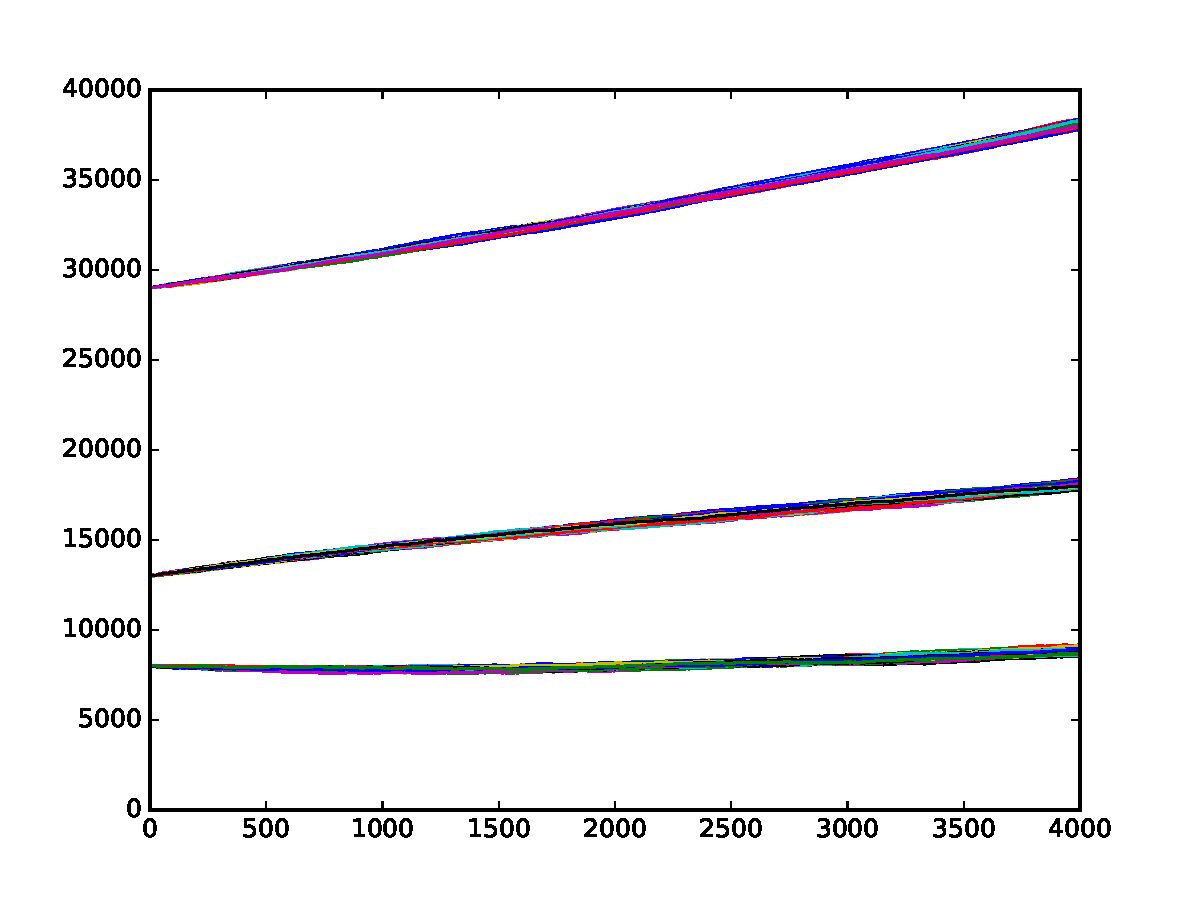
\includegraphics[width=\textwidth]{figures/raw_data_disease_free.pdf}
		\caption{Raw data from a set of realisations on a system without disease. Note how all runs seem to be fairly similar.} \label{fig:results:raw_no_disease}
	\end{subfigure}
	\begin{subfigure}{0.45\textwidth}
		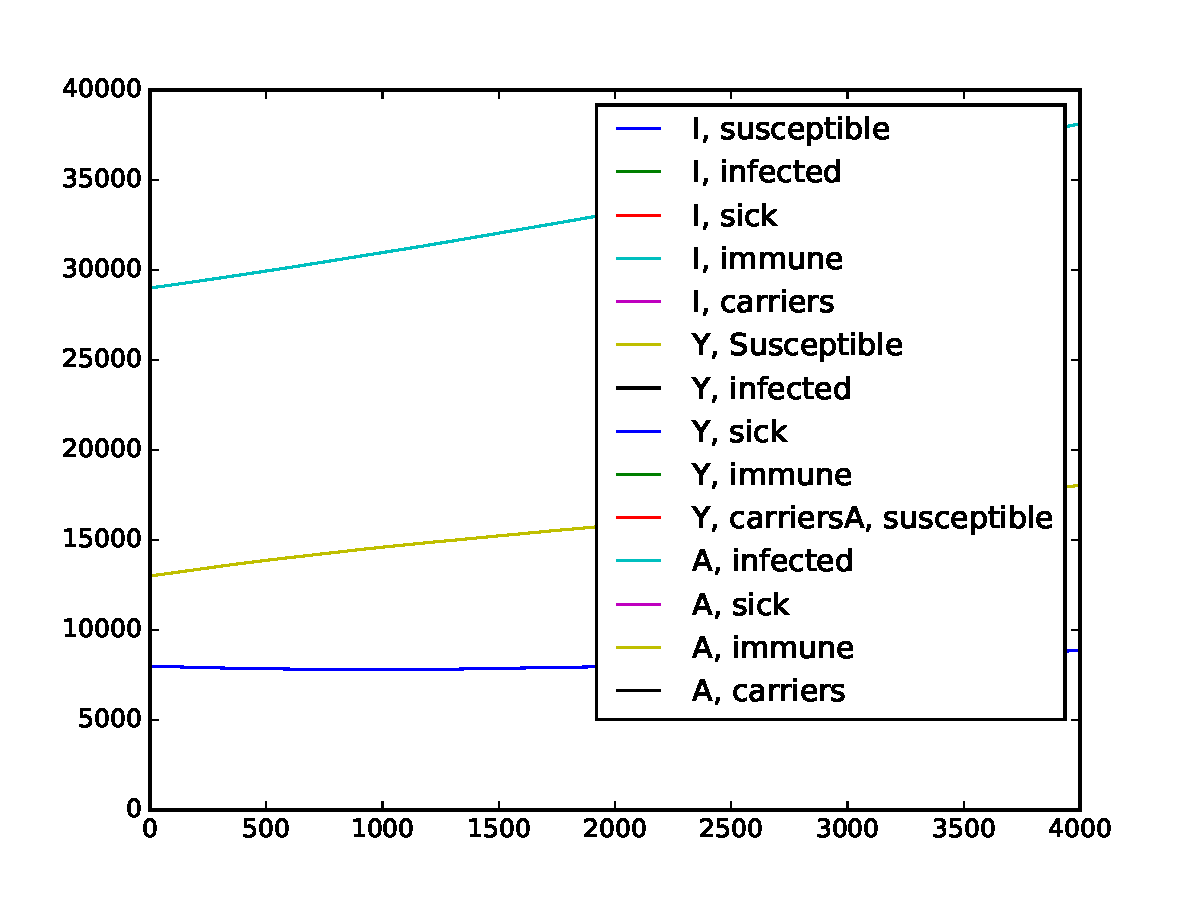
\includegraphics[width=\textwidth]{figures/plotted_aves_disease_free.pdf}
		\caption{Average of the runs shown in \cref{fig:results:raw_no_disease}.} \label{fig:results:ave_no_disease}
	\end{subfigure}
	\caption{Basic data sets for a set of realisations of a system without disease. Right is an average of the simulations on the left.} \label{fig:results:no_disease}
\end{figure}

We also consider the validity of the model after the introduction of endemic disease for two different serotypes. The results are shown in \cref{fig:results:endemic_disease}. The primary goal of this simulation is to examine whether the model could mimic the endemic behaviour of the disease, with the appropriate number of disease cases and carriers. The results from these runs are similar to the available results from field research for both serotypes. However, note that there is no significant ratio of immune individuals of any age group for the system with serogroup W-135, as carriage of that strain does not induce immunity. 

\begin{figure}[h]
	\centering
	\begin{subfigure}{0.45\textwidth}
		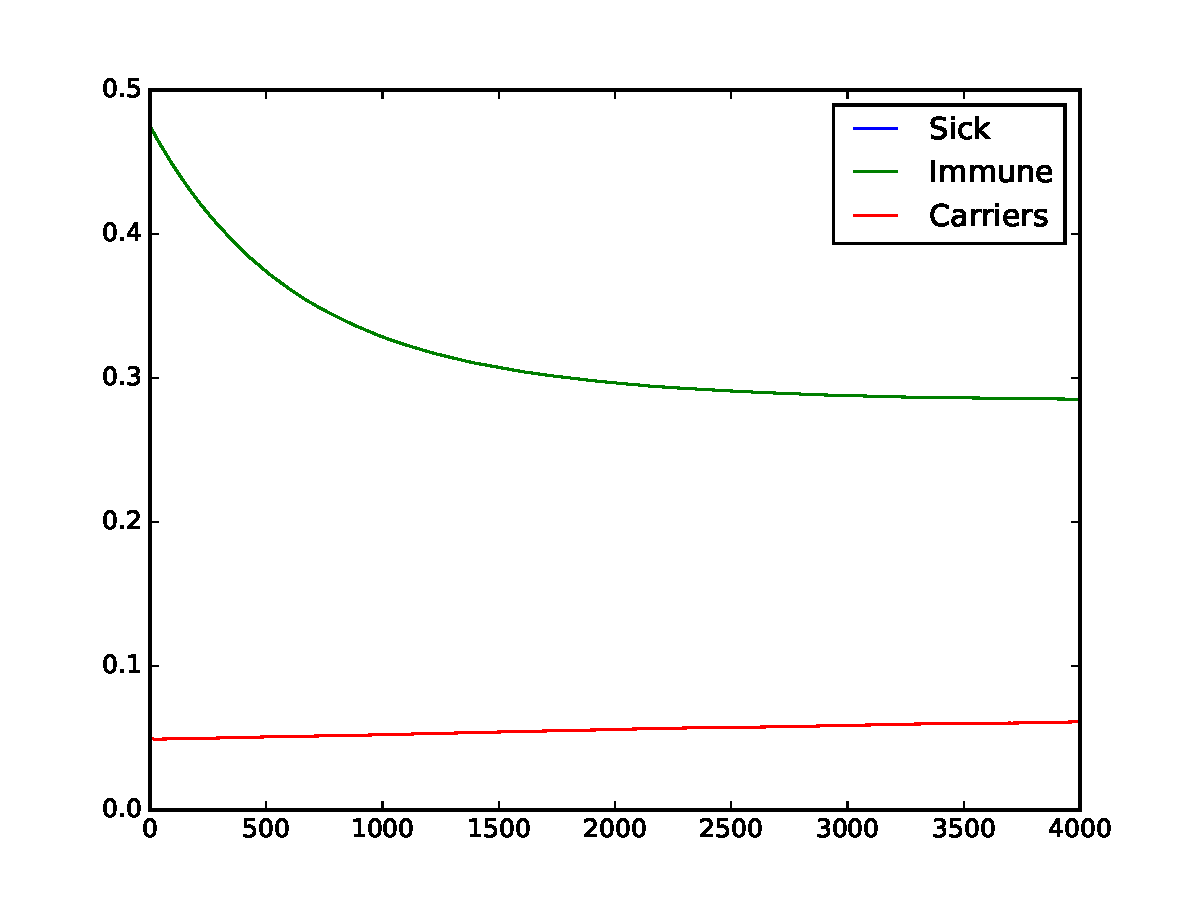
\includegraphics[width=\textwidth]{figures/plotted_disease_endemic_1pop_A.pdf}
		\caption{Average of one set of runs on a system with parameters matching disease of serogroup A in an endemic state. No seasonal variations were introduced in these simulations.} \label{fig:results:endemic_disease_A}
	\end{subfigure}
	\begin{subfigure}{0.45\textwidth}
		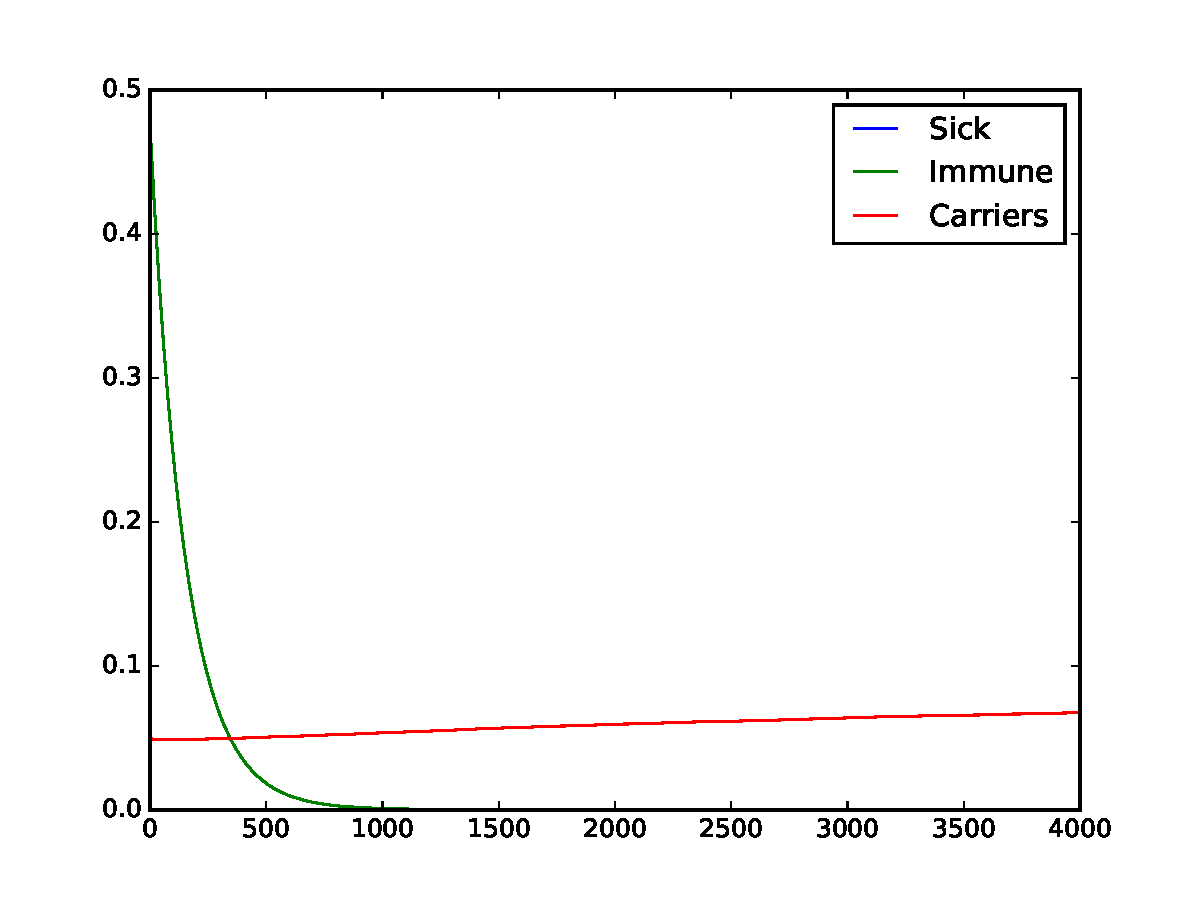
\includegraphics[width=\textwidth]{figures/plotted_disease_endemic_1pop_W135.pdf}
		\caption{Average of one set of simulations on a system with parameters matching disease of serogroup W-135 in an endemic state. No seasonal variations were introduced in these simulations.} \label{fig:results:endemic_disease_W135}
	\end{subfigure}
	\caption{Figures showing the results from simulation for a system with parameters matching two different serotypes of disease. Overall, the results are similar except in the subpopulations of immune individuals. Immunity is lacking from all age groups for the system corresponding to serogroup W-135} \label{fig:results:endemic_disease}
\end{figure}

Considering the model with disease included, it is important to note that the parameter governing the transmission of disease was used to have the system match the data, due to lack of available research. A common estimate of the parameter $R_0$ was produced using a set of simulations, and the value producing the best correspondence to real data was chosen. As such, these results are not as reliable as would be desired.



\subsection{Seasonal variations}

The seasonal variations in number of disease cases was postulated to have two possible explanations, and both of these are examined in this section. First we consider an explanation from behavioural changes, and then an explanation from the biology of the bacterium itself. It is worth commenting that in the second case, the parameter can be controlled so that the data matches reality, as the parametrization is dependent on the model itself. Only a negative result would be significant here, as it means that the model can not be applied to this case. Validation of this theory must come from some other source.

\subsubsection{Behavioural changes}

A graph showing the seasonal variations in disease cases for this type of run is shown in \cref{fig:results:seasonal_disease}. It is clear from the graphs that there are significant differences between the different seasons. The weekly incidence rates reflects these variations, and show a significant differnce between the dry and the wet season. However, the increase in incidence rate does not reflect the shift from endemic to hyperendemig incidence rates presented in the introduction. Including even larger differences between the population density in the dry and the wet season would most likely be able to correct for this discrepancy, if it is found that the population behaviour corresponds to a larger migratory pattern.

The more interesting result for these runs are the carrier rates, which are about four times larger than what is produced for a run without seasonal changes. This difference can be seen both during the wet season and the dry season. The increase during the dry season is explained by the increased rate of disease spread during this time, and as the expected duration of carriage is so long this will also affect the ratios during the wet season.

\begin{figure}
	\centering
	\begin{subfigure}{0.45\textwidth}
		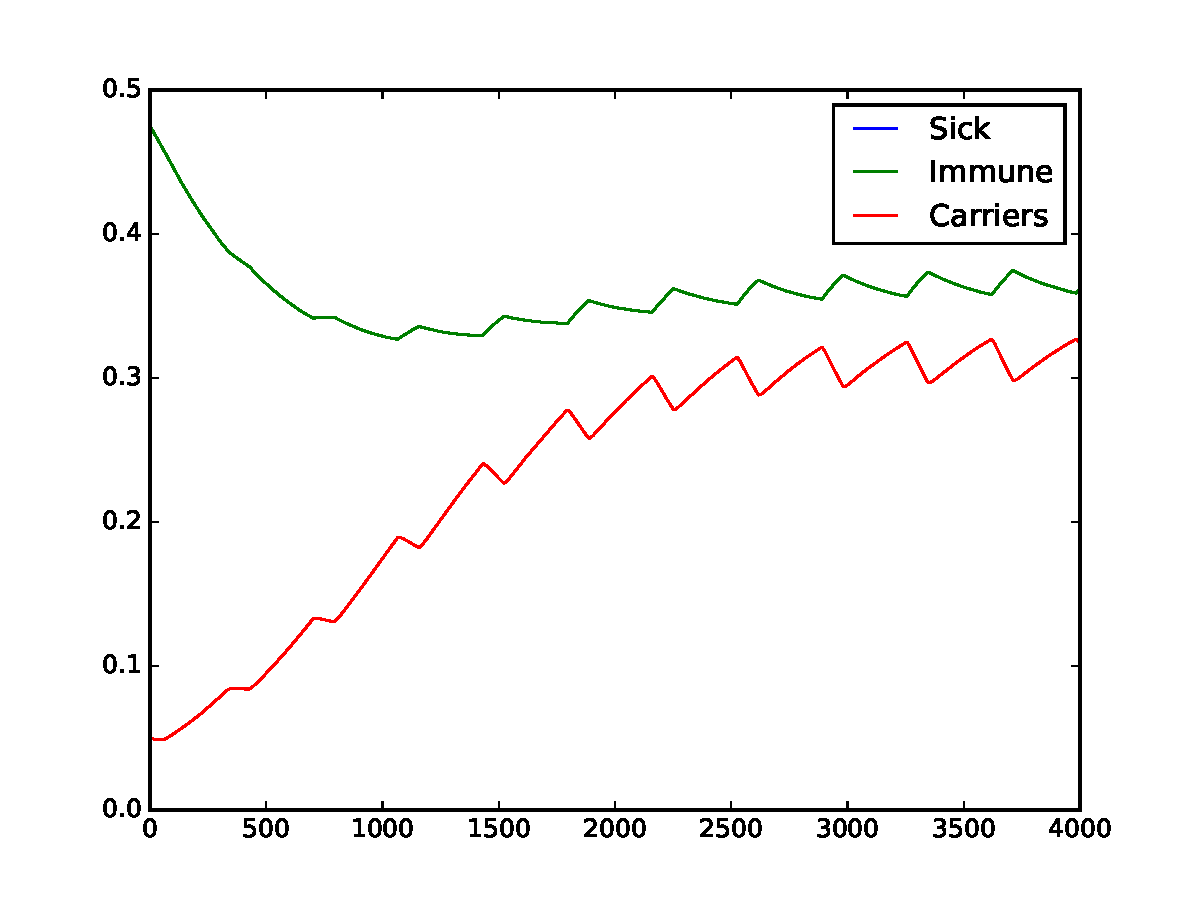
\includegraphics[width=\textwidth]{figures/plotted_disease_endemic_2pop_A}
		\caption{Graph showing some tdata for a system corresponding to a population with seasonal behavioural variations, subject to disease of serogroup A. Displayed are the ratios of the population in all age groups that are immune, carriers or sick. The seasonal variations in the ratio of immune and carriers are very clear. The ratio of sick is too small to be seen in this plot, and incidence rates are presented elsewhere. The carriage rates for this system are significantly higher than in the system without seasonal variations.} \label{fig:results:seasonal_disease_A}
	\end{subfigure}
	\begin{subfigure}{0.45\textwidth}
		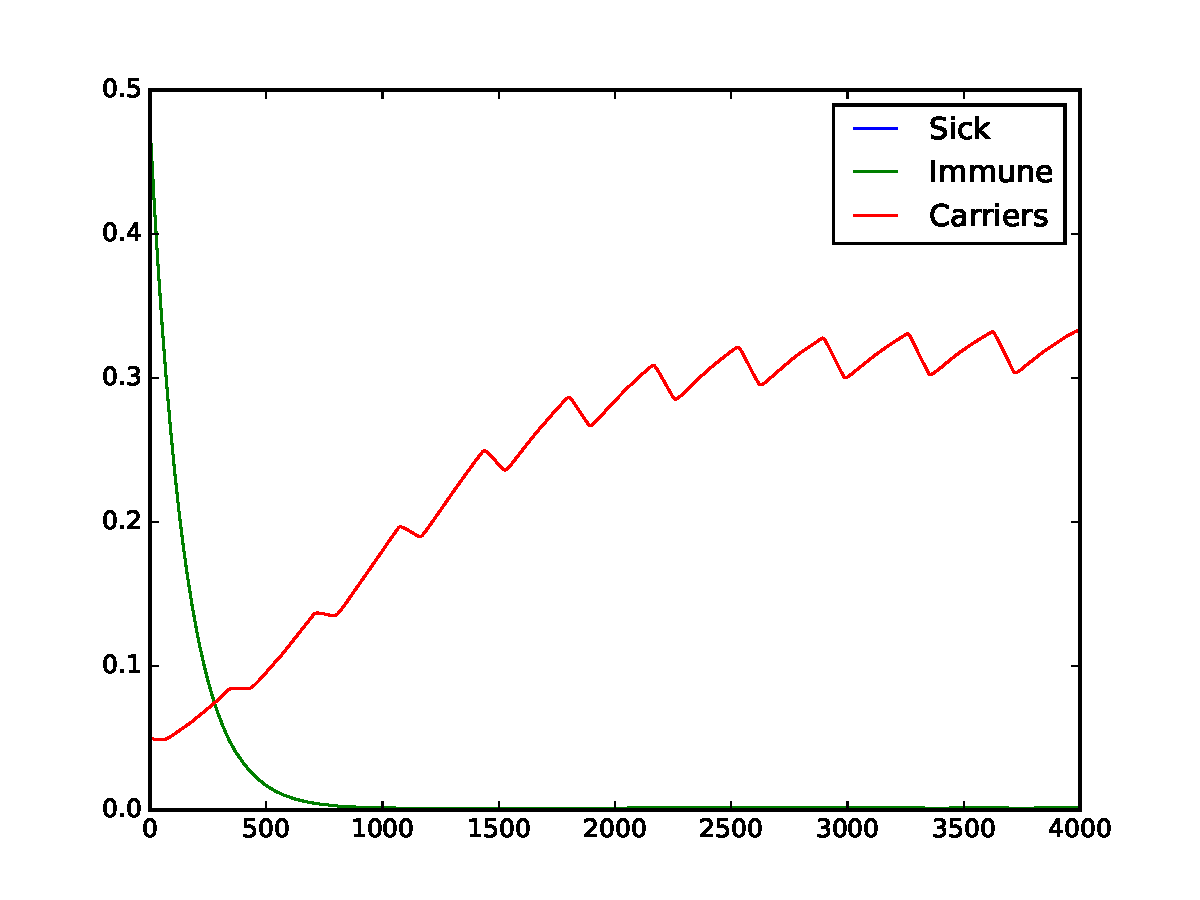
\includegraphics[width=\textwidth]{figures/plotted_disease_endemic_2pop_W135}
		\caption{Graph showing some data for a system corresponding to a population with seasonal behavioural variations, subject to disease of serogroup W-135. Diseplayed are the ratios of the population in all age groups that are immune, carriers or sick. The seasonal variations in the ratio of carriers are very clear, but the ratio of immune and sick individuals are not significant enough to be seen in this graph (after transient behaviour). The carriage rate is significantly higher in this system than in the corresponding system without seasonal variations.} \label{fig:results:seasonal_disease_W135}
	\end{subfigure}
	\caption{Figures showing some data for systems corresponding to seasonal variations caused by behavioural changes, for the two serogroups considered in this project. The two systems are similar other than in the ratio of immunity. Also not the significant higher carriage rates overall compared to \cref{fig:results:endemic_disease}} \label{fig:results:seasonal_disease}
\end{figure}

These results do not differ significantly between the serogroups examined. The results that do differ is again the immunity rates, where there is no significant population immunity against serogroups W-135. As the remaining results are so similar, it is reasonable to assume that population immunity does not in general affect the difference between the endemic and hyperendemic states.

\subsubsection{Parametrical changes}
% Seasonality modelling
%			- population grouping on season
%			- different parameters
%				- comparison

\subsection{Epidemics}
% Epidemics modelling
%		- I don't know what the results are yet here ^^

% Memo: Look at all immune groups, including permanent immunity
% Look at the number of disease cases -> events, not population numbers

% CLIPPED FROM GOALS

% The primary goal of this project has been to create and implement stochastic model for the population and disease dynamics in the African Meningitis belt. The model should be evaluated, and its calculations should be compared to real-world data and other models, to determine whether there is an improvement in the accuracy and specificity of the model.

% If the model and its implementation seems sound, some further questions are to be considered. The primary consideration of this thesis is to attempt to determine whether the difference between the endemic and the hyperendemic states of the disease can be explained by behavioural changes or whether the explanation must be found somewhere else, for example in biochemical factors of the bacterium itself.

% To further determine the seasonality of the disease, also the epidemic state should be considered. While epidemic outbreaks are connected to the introduction of a more invasive strain, the epidemics themselves also display a certain seasonality. Using the seasonal variations found to produce the most accurate results in the previous section, the results of introducing a more invasive strain during different seasons will be examined. If the introduction leads to an epidemic also during the wet season, or fails to lead to an epidemic in the dry season, the suggested explanation does not hold.

\section{Conclusions}

DISCUSSION POINTS \\
 - Possible improvements of the implementation \\
 - Possible risks with non-specific individuals \\
 - Uncertainty in the parameters \\
 - Uncertainty in the carriage rates \\
 - Cross immunity \\
 - Immunity affecting carriage \\
 - Quantative vs qualitative statements


% Figure float, including 2 subfigures
%\begin{figure}
%	\centering
%	\begin{subfigure}{0.45\textwidth}
%		\includegraphics[width=\textwidth]{}
%		\caption{} \label{}
%	\end{subfigure}
%	\begin{subfigure}{0.45\textwidth}
%		\includegraphics[width=\textwidth]{}
%		\caption{} \label{}
%	\end{subfigure}
%	\caption{} \label{}
%\end{figure}

%\begin{wrapfigure}{r}{0.5\textwidth}
%	\includegraphics[width=0.48\textwidth]{}
%	\caption{} \label{}
%\end{wrapfigure}

\newpage

\begin{appendices}

%\lstinputlisting[language=matlab, style=matlab_custom]{} % Example code input

\end{appendices}

\bibliographystyle{plain}
\bibliography{bibliography}


\end{document}